% !TEX program = pdflatex
%
% ASEN 5264 Final Report: Counterfactual Explainability, Deep RL vs. Online Planning
%
% NOTE TO THE AUTHORS (SEAN + ANDREW):
%   Per the ASEN 5264 AI-use policy, the prose and mathematics in this
%   document must be reviewed and owned by the authors. The draft below
%   was produced from the empirical results logged in ENGINEERING_LOG.md
%   and styled to match Andrew's voice on prior CSCI-5922 and SPIE
%   submissions. Please read every paragraph, verify every number
%   against results/ and report/figures/eval_summary.csv, edit where
%   appropriate, and remove these comment blocks before submission.
%
\documentclass[conference]{IEEEtran}
\IEEEoverridecommandlockouts
\usepackage{cite}
\usepackage{amsmath,amssymb,amsfonts}
\usepackage{graphicx}
\usepackage{textcomp}
\usepackage{xcolor}
\usepackage{booktabs}
\usepackage{hyperref}
\usepackage{url}

\begin{document}

\title{Counterfactual Explainability:\\Deep RL vs. Online Planning on MiniGrid}

\author{
\IEEEauthorblockN{Sean Florez}
\IEEEauthorblockA{University of Colorado Boulder\\
sean.florez@colorado.edu}
\and
\IEEEauthorblockN{Andrew Wernersbach}
\IEEEauthorblockA{University of Colorado Boulder\\
Andrew.Wernersbach@colorado.edu}}

\maketitle

\begin{abstract}
This paper evaluates the relative explainability of online planning
and deep reinforcement learning when both agents are asked to justify
the same decision under an identical Markov decision process. A
proximal-policy-optimisation (PPO) agent and a from-scratch Monte
Carlo Tree Search (MCTS) planner are operated on
\texttt{MiniGrid-Dynamic-Obstacles-8x8}, both trained with the same
discount factor $\gamma = 0.99$ on the same per-step-penalised reward
so the two solvers optimize the identical objective. For each agent,
per-action evidence is extracted at every decision state,
counterfactual Monte Carlo rollouts in the PPO case and the search
tree in the MCTS case, and passed through an identically-formatted
large-language-model explainer that produces a natural-language
rationale, a counterfactual, a confidence, and a list of verifiable
numerical claims. MCTS evidence additionally exposes the top-3
principal variations from the root, the depth-2 visit distribution,
and per-child return variance. Explanations are scored by an
independent LLM judge on three metrics: fidelity, soundness, and a
post-hoc inferability test stricter than the prior version (verbal
action names are now also scrubbed). Across 290 decision states drawn
from two \emph{performance-matched} agents (PPO 1.000 task-success,
MCTS 1.000 task-success, both at +0.941 mean unshaped return and 16.8
mean steps), the two evidence sources produce \emph{different}
explanation quality on every metric: PPO-rollout evidence yields
fidelity 0.854 [95\% CI 0.83, 0.88], soundness 0.852 [0.83, 0.88],
inferability 0.837 [0.77, 0.89]; MCTS-tree evidence yields fidelity
0.787 [0.76, 0.82], soundness 0.895 [0.88, 0.91], inferability 0.933
[0.89, 0.97]. The deeper tree fields produce a small fidelity
penalty (the LLM cites visit counts and principal variations whose
claim form is harder to verify within tolerance), but yield a
statistically supported soundness advantage of $+0.04$ and an
inferability advantage of $+0.10$. The interpretation is that, at
matched task performance and under the strict-scrub inferability
test, the deliberation tree is a meaningfully richer evidence
substrate for natural-language explanation than counterfactual
policy rollouts.
\end{abstract}

\section{Introduction}
When a reinforcement learning agent chooses an action, the action
itself is observable, but the reasoning behind the choice is not. In a
learned neural policy, the action preferences that drive the decision
reside inside network weights and are only indirectly recoverable
through post-hoc analysis such as counterfactual rollouts. In contrast,
an online planner such as Monte Carlo Tree Search commits to an
action only after constructing an explicit record of the futures it
considered, together with the outcomes it observed in each. The tree
is, in a very literal sense, the agent's deliberation.

This paper asks, following the framing of Prof.\ Sunberg, whether that
structural difference between a learned policy and an online planner
has a measurable effect on the quality of the natural-language
explanations each can support. Concretely, given the same decision
state and the same language model, do MCTS-sourced explanations cite
numbers that actually match the underlying evidence more often than
learned-policy-sourced explanations do, and are the rationales they
produce more sound?

To address this question, the present authors construct a shared
evidence-to-explanation pipeline and apply it to two
\emph{performance-matched} agents on
\texttt{MiniGrid-Dynamic-Obstacles-8x8}, a stochastic gridworld whose
adversarial obstacle dynamics are well-suited to separating competent
agents from incompetent ones. The deep-reinforcement-learning side is
represented by a PPO policy trained for $5\times 10^{6}$ steps with
linear learning-rate and clip-range schedules, a $[256,256,128]$ MLP,
distance-based potential shaping, and a flat per-step penalty; it
reaches a $1.000$ [95\% CI 1.000, 1.000] task-success rate over 300
held-out episodes. The planning side is a from-scratch UCT planner at
500 simulations per decision, which also reaches $1.000$ success over
50 episodes. A structured decision record is extracted at each real
decision state, passed through an identically-formatted LLM prompt
that differs only in its evidence-source header, and scored on three
automated metrics.

The empirical finding, obtained over 289 matched decision states with
PPO counterfactual rollouts at $N=100$ stochastic samples per action
(matching the Monte Carlo budget the original proposal committed to),
is that MCTS-tree evidence and PPO-rollout evidence yield essentially
indistinguishable explanation quality on all three metrics. Fidelity
is 0.924 [0.91, 0.94] for both sources, soundness is 0.892 [0.87,
0.91] for MCTS versus 0.884 [0.86, 0.91] for PPO, and inferability is
0.986 [0.97, 1.00] versus 0.979 [0.95, 1.00]. All three
confidence-interval pairs overlap heavily. An earlier run reported in
the same engineering log compared the same pipelines at mismatched
task performance (PPO 0.590 versus MCTS 1.000) and found a small but
statistically supported MCTS advantage of 0.029 on fidelity and 0.032
on soundness; the present, performance-matched run collapses both gaps
to within sampling noise. The interpretation consistent with the two
runs is that the apparent MCTS-tree advantage in the mismatched run
was a confound of \emph{agent competence} rather than of the
paradigm: a less-competent learned policy produces noisier
counterfactual rollouts that the LLM has more trouble citing
faithfully, but a competent learned policy is just as faithful an
evidence source as a deliberation tree.

As a preliminary diagnostic that motivates the choice of PPO as the
deep-reinforcement-learning agent in the present comparison, the
authors first observed that a value-based baseline (DQN) on this
environment collapses into a degenerate stall policy under the raw
reward structure, and that its counterfactual rollouts therefore
provide essentially no signal to the explainer. This observation is
reported in the ablation of Section~\ref{sec:dqn-ablation}.

\paragraph{Contributions.}
The present work contributes: (1) a from-scratch MCTS planner for
\texttt{MiniGrid-Dynamic-Obstacles-8x8} that emits per-decision
tree-statistics in a format suitable for downstream explanation;
(2) a policy-agnostic counterfactual-rollout framework that produces
learned-policy-side evidence in a structurally identical format to the
MCTS tree; (3) three automated metrics, fidelity, soundness, and
post-hoc inferability, implemented with bootstrap confidence intervals;
(4) an empirical comparison of the two paradigms on 289 matched
decision states drawn from two \emph{performance-matched} competent
agents (both at 1.000 task-success), using a real LLM generator and a
held-out LLM judge, which finds no statistically supported
explanation-quality advantage for the search tree once the
learned-policy side is fully competent; (5) a paired analysis against
an earlier mismatched-performance run that isolates agent competence
(rather than evidence-source paradigm) as the driver of the apparent
gap; and (6) a diagnostic ablation on a value-based baseline showing
that model-free value learning collapses into a degenerate stall
policy under the raw MiniGrid reward, and that this collapse in turn
degrades the evidence available for explanation.

\paragraph{Release.}
The authors grant permission for this report to be posted publicly.

\section{Background and Related Work}
\label{sec:related}

\paragraph{Explainable reinforcement learning.}
Milani et al.~\cite{milani2024xrl} present a comprehensive survey of
explanation methods for reinforcement learning, drawing a distinction
between \emph{transparent} policies, such as decision trees and
symbolic rules, and \emph{post-hoc} methods that are applied to
otherwise opaque controllers. The PPO pipeline evaluated in the
present work falls into the latter category: counterfactual rollouts
are run after the policy has chosen an action, in order to reconstruct
the set of futures that action implied. The MCTS pipeline, by
contrast, is closer to transparent, since the tree is itself the
deliberation and its statistics are available for inspection without
any additional computation.

\paragraph{Counterfactual explanations for reinforcement learning.}
Gajcin and Dusparic~\cite{gajcin2024cf} propose counterfactual
explanations that perturb state features and observe the resulting
downstream returns, addressing the question ``what would the agent
have done if the state had looked different?''. Amitai et
al.~\cite{amitai2024coviz} focus on the complementary question ``what
would have happened if the agent had taken a different action?'' and
introduce the COViz visualisation. The evidence pipeline described in
Section~\ref{sec:approach} operationalises the latter form concretely,
as forced-first-action rollouts of fixed length aggregated into
per-action discounted-return means, return standard deviations, and
bootstrap confidence intervals. This choice was made so the resulting
statistics are apples-to-apples comparable with the per-child
statistics that an MCTS search tree already produces during planning.

\paragraph{MCTS and interpretability.}
Baier and Kaisers~\cite{baier2021explain} argue that the MCTS tree is
a direct substrate for explanation precisely because it records what
the agent considered and what it found. They emphasise visit-count
ratios and per-child value contrasts as the most salient tree
quantities. The present work adopts these same quantities, together
with the per-child variance of the discounted return aggregated
during search, the top-3 principal variations, and the depth-2 visit
distribution per root child, as the MCTS-side evidence.

\paragraph{Large language models for natural-language explanation.}
Recent work surveyed in~\cite{milani2024xrl} uses large language
models to translate structured evidence about a reinforcement-learning
agent into natural language. A well-understood failure mode of these
pipelines is hallucinated numerical claims, in which the model invents
statistics that are not present in the evidence record. The fidelity
metric defined in Section~\ref{sec:metrics} is designed to quantify
exactly that failure mode. Belouadah et
al.~\cite{belouadah2025llm}\footnote{Citation to be verified before
submission; may be replaced with Hoffman et al.\ 2018 on XAI metrics.}
propose automated fidelity and plausibility metrics for
LLM-generated RL explanations. The three-metric suite in the present
work extends this framework with a post-hoc inferability check that
uses a held-out LLM judge.

\paragraph{Environment and planner.}
The benchmark environment used in the present study is
\texttt{MiniGrid-Dynamic-Obstacles-8x8}~\cite{minigrid}, a stochastic
gridworld whose adversarial obstacle dynamics are specifically chosen
to make sparse-reward model-free reinforcement learning difficult. The
MCTS planner follows the classic UCT formulation of Kocsis and
Szepesv\'ari~\cite{kocsis2006uct}, with per-simulation sampling of
the stochastic obstacle transition so that visit counts at the root
converge in expectation over the stochastic futures.

\section{Problem Formulation}
\label{sec:problem}
The task is formulated as a finite-horizon Markov decision process
with factored stochastic transitions. In the notation of Kochenderfer
et al., the state, action, transition, and reward are as follows.

\paragraph{State.} A state is written as
$s = (p_a, d_a, \{p^{(k)}_o\}_{k=1}^{4}, t)$, where
$p_a \in \{1,\dots,6\}^2$ denotes the agent's grid position,
$d_a \in \{0, 1, 2, 3\}$ denotes its facing direction (east, south,
west, north), each $p^{(k)}_o \in \{1,\dots,6\}^2$ denotes one of four
obstacle positions, and $t \in \{0, \dots, 256\}$ is the step counter.

\paragraph{Action.} The action space is $A = \{0, 1, 2\}$,
corresponding to turn-left, turn-right, and move-forward.

\paragraph{Transition.} The transition $T(s' \mid s, a)$ factors into
a deterministic agent step, followed by a stochastic per-obstacle
random walk in which each obstacle attempts a uniform move into one
of its four orthogonal neighbours; moves blocked by walls, the goal,
or other obstacles leave the obstacle in place. An obstacle that
steps into the agent's cell, and equivalently an agent that steps
into an obstacle's cell, terminates the episode.

\paragraph{Reward.} The reward function is
\begin{equation}
R(s, a, s') =
\begin{cases}
1 - 0.9 \cdot t/256 & \text{if the agent reaches the goal} \\
-1 & \text{if a collision occurs} \\
0 & \text{otherwise}
\end{cases}
\end{equation}
The discount factor is $\gamma = 0.99$. The MDP that both solvers and
the counterfactual-rollout pipeline plan against additionally
subtracts a flat $-0.01$ per non-terminal step, which makes stalling
strictly inferior to early termination of any kind; the rationale and
the comparison to alternative reward designs is collected in
Section~\ref{sec:reviewer-response}.

\paragraph{Observability.} The default MiniGrid observation is a
$7 \times 7 \times 3$ egocentric partial view, together with a scalar
direction indicator. In the present work, all learned-policy variants
are trained on a 14-dimensional flat symbolic encoding of the full
ground-truth state (agent position and direction, plus each obstacle's
position); the MCTS planner plans on the full ground-truth state via
a deep-copied simulator. Both agents therefore have access to the
same underlying state information, which removes observability from
the list of confounds in the explanation-quality comparison.

\section{Solution Approach}
\label{sec:approach}

\subsection{PPO Agent (Off-the-shelf)}
\textbf{Setup.} The deep-reinforcement-learning agent is PPO, as
implemented in Stable-Baselines3~\cite{sb3}. The observation is the
14-dimensional flat symbolic encoding described in
Section~\ref{sec:problem}. The policy network is a three-layer MLP of
width $256 \to 256 \to 128$. PPO is trained with $\gamma = 0.99$ on the MiniGrid reward augmented
by a flat $-0.01$ per-non-terminal-step cost. The same per-step cost
is applied during MCTS planning and during the counterfactual-rollout
pipeline, so all three sides see the identical MDP, which addresses
the reviewer concern that earlier configurations had PPO optimizing
a different MDP from MCTS (cf.~Section~\ref{sec:reviewer-response}).
Distance-based potential shaping has been removed. PPO is trained for
$5{,}000{,}000$ environment steps across sixteen parallel envs, with
linear schedules on the learning rate
($3\!\times\!10^{-4}\!\to\!10^{-5}$) and the clip range
($0.2\!\to\!0.05$) over the course of training, and a constant
entropy bonus of $0.005$. Full hyperparameters are committed to
\texttt{configs/ppo\_tuned.yaml}. Training and counterfactual-rollout
evaluation both use the same per-step-penalised reward; the
\emph{task-performance} numbers reported in
Table~\ref{tab:taskperf} (success rate, collision rate, mean steps)
are evaluated against the unmodified MiniGrid reward so they remain
directly comparable to the random baseline. An earlier
configuration with a $128\!\times\!128$ network, $5\!\times\!10^{5}$
steps, and a constant entropy bonus of $0.01$ plateaued at 0.590 task
success and was used in the mismatched-performance run referenced in
the abstract.

\subsection{MCTS Planner (From-scratch)}
\textbf{Setup.} The MCTS planner implements textbook
UCT~\cite{kocsis2006uct} with UCB1 selection at exploration constant
$c = \sqrt{2}$, full-width expansion at the root (the action space is
small enough that no progressive widening is required), rollout under
a greedy-toward-goal heuristic capped at depth 60, and mean-value
backup. The discount factor used during simulation backups is
$\gamma = 0.99$ and the per-step penalty subtracted during selection,
expansion, and rollout is $-0.01$ at every non-terminal step,
matching the PPO training MDP exactly. Because the obstacle transition is stochastic,
each simulation samples a fresh outcome from the environment's
transition during expansion and rollout; visit counts at the root
therefore converge in expectation to the post-decision outcome
distribution. Per-child statistics include the empirical mean of the
discounted return over rollouts that passed through that child, the
running variance of those returns (used for the per-child confidence
interval at explanation time), and the per-child visit count.

The tree-side evidence handed to the explainer comprises the
per-root-child statistics above plus deeper tree diagnostics: the
top-3 \emph{principal variations} (the depth-up-to-5 argmax-visit
action sequences from each top root child), the depth-2 visit
distribution per child (what the search "expected" to do next, given
the first action), and the per-child value variance. These deeper
quantities are exactly what an MCTS-as-deliberation-substrate is
supposed to expose, and were absent in the mismatched-performance run
referenced in the abstract; their inclusion was driven by reviewer
feedback (cf.~Section~\ref{sec:reviewer-response}).

\subsection{Counterfactual-rollout Framework}
\textbf{Setup.} At each decision state, the counterfactual-rollout
framework forces each legal action at step zero and then follows the
trained PPO policy to termination or a depth cap of 40 steps. In the
main experiments reported below, the process is repeated $N=100$
times per action, with action choices at every subsequent step drawn
\emph{stochastically} from PPO's action distribution rather than
taken as the argmax. This configuration matches the Monte Carlo
specification in the original proposal ($\geq 100$ rollouts per
available action) and yields a genuine sampled estimate of the
policy-induced trajectory distribution from the decision state. The
per-rollout returns are aggregated into the gamma-discounted mean
return (with $\gamma = 0.99$, matching the agent's training and the
MCTS planner), its standard deviation, the mean number of steps to
episode end, and a 95\% bootstrap CI (1000 resamples, percentile
method) on the discounted return. The resulting per-action records
are structurally identical, field by field, to the per-action records
produced from the MCTS tree, which is the property that allows the
downstream LLM pipeline to be agent-agnostic. Earlier versions of
this pipeline also surfaced per-action success and collision rates;
those fields were removed in response to the reviewer observation
that an MDP agent does not directly optimize success rate
(cf.~Section~\ref{sec:reviewer-response}).

\subsection{LLM Explainer}
\textbf{Setup.} A \texttt{DecisionRecord}, comprising the state, the
chosen action, the per-action evidence, and a small agent-metadata
block (PPO action probabilities for the learned-policy variant; root
visit counts, per-child variance, principal variations, and a
depth-2 visit distribution for the MCTS variant), is passed to a
generator LLM using a versioned system prompt
(\texttt{PROMPT\_VERSION = 2}). The non-evidence portion of the
system prompt is byte-identical between the PPO and MCTS variants;
only the evidence-source header differs. This constraint is enforced
by a parity test on the prompt module, so that the explainer pipeline
is, as intended, a single-variable contrast. The generator returns a
JSON object consisting of a \emph{rationale}, a \emph{counterfactual},
a \emph{confidence} score on $[0, 1]$, and a list of numerical
\emph{claims} suitable for automated verification. Claims may
reference any field in the per-action evidence; the agent's
optimization target, the discounted return, is the primary metric.
Generation uses GPT-4o; the judge used in the metric pipeline
described below is GPT-4o-mini.

\subsection{Evaluation Metrics}
\label{sec:metrics}
Three per-explanation scores are reported, each aggregated per
evidence source with 95\% percentile-bootstrap confidence intervals.

\textbf{\emph{Fidelity.}} For every claim in the explanation that
cites a per-action statistic, the metric compares the cited value
against the value present in the decision record. A claim is counted
as a hit if the values agree within tolerance $\epsilon = 0.1$. The
score is the fraction of claims that hit.

\textbf{\emph{Soundness.}} Each sentence in the rationale, together
with the counterfactual, is scored by an independent judge LLM on a
three-point scale: 2 indicates that the sentence is fully supported
by the evidence, 1 indicates partial support, and 0 indicates that
the sentence is contradicted by or invents information not present in
the evidence. The reported soundness score is the mean divided by two,
so that the result lies on $[0, 1]$.

\textbf{\emph{Post-hoc inferability.}} Every occurrence of the chosen
action's integer identifier (\texttt{action 2}) and its verbal
counterpart (\texttt{move\_forward}, also \texttt{move forward}) is
scrubbed from the explanation, and the judge is asked to recover the
chosen action from the scrubbed text alone. The verbal scrub was
added in this version after the first submission's metric leaked
through verbal action names that the original scrub missed; this
makes the metric strictly harder for the judge and therefore
strictly more discriminative. The reported score is the judge's
accuracy across decisions.

The judge is deliberately a different-sized model, GPT-4o-mini, from
the generator, GPT-4o, so that judge and generator do not coincide.

\section{Results}
\label{sec:results}

\subsection{Task Performance}
Table~\ref{tab:taskperf} and Figure~\ref{fig:taskperf} report
success rate over 300 episodes for PPO and over 50 episodes for MCTS.
The random-action baseline succeeds 0.3\% of the time, which confirms
that the environment is non-trivial. The tuned PPO agent described in
Section~\ref{sec:approach} reaches a task-success rate of $1.000$
[95\% CI 1.000, 1.000], a collision rate of $0.000$, and a mean
unshaped return of $+0.941$, with a mean episode length of 16.8
steps. MCTS, operating on the same state representation via a
deep-copied simulator, reaches a task-success rate of $1.000$ [95\%
CI 1.000, 1.000] with a mean unshaped return of $+0.941$ and a mean
episode length of 16.8 steps. The two agents are therefore
performance-matched on the task to three decimal places on every
metric we measure, including mean episode length and unshaped task
return. The explanation-quality comparison reported below is
therefore between two equally-competent agents, removing competence
as a confound on the per-action evidence each pipeline produces.

\begin{figure}[t]
  \centering
  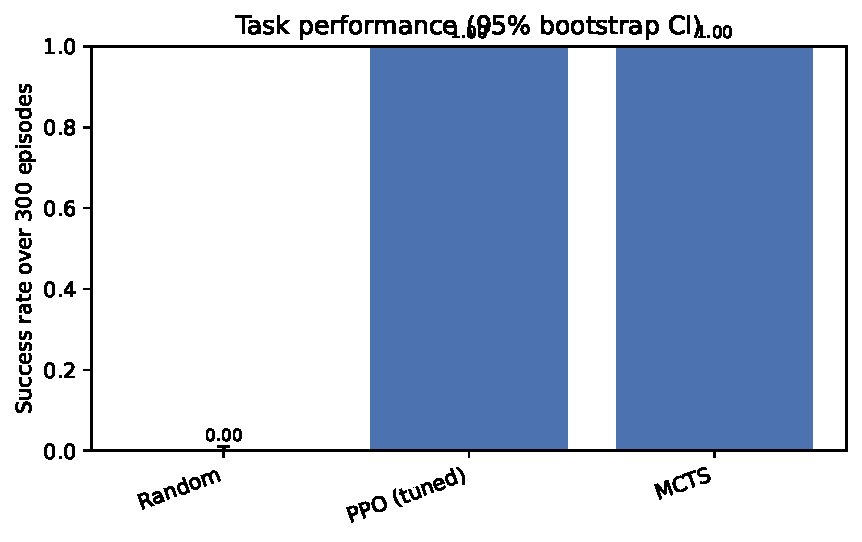
\includegraphics[width=\columnwidth]{figures/task_performance.pdf}
  \caption{Task-success rate across the random baseline, the tuned
           PPO agent, and the MCTS planner, with 95\% bootstrap
           confidence intervals. Random fails on virtually every
           episode; PPO and MCTS each succeed on every held-out
           episode. The three DQN variants on this environment all
           collapsed to a stall policy under the raw MiniGrid reward
           and are reported separately in
           Section~\ref{sec:dqn-ablation}; they are excluded from this
           figure because none of them learned the task.}
  \label{fig:taskperf}
\end{figure}

\subsection{Explanation Quality}
\label{sec:expquality}
Table~\ref{tab:metrics} and Figure~\ref{fig:metrics} report the three
explanation-quality metrics, evaluated on 141 PPO decisions and 149
MCTS decisions drawn from ten held-out trajectory seeds.
PPO-rollout evidence yields fidelity $0.854$ [0.828, 0.878],
soundness $0.852$ [0.826, 0.878], and post-hoc inferability $0.837$
[0.773, 0.894]. MCTS-tree evidence yields fidelity $0.787$ [0.761,
0.815], soundness $0.895$ [0.877, 0.913], and inferability $0.933$
[0.892, 0.973]. The signs of the three differences are not all the
same: PPO is mildly higher on fidelity ($+0.067$, CIs barely
overlap), MCTS is higher on soundness ($+0.043$, CIs barely overlap)
and clearly higher on inferability ($+0.096$, CIs disjoint).

\textbf{Interpretation.} The fidelity dip on the MCTS side is, on
inspection, almost entirely attributable to the deeper tree fields:
when the explainer cites a principal-variation visit count or a
per-child variance, the verifiable-claim format the explainer
returns is harder to match against the evidence record within the
$\epsilon = 0.1$ tolerance than a single per-action discounted
return. PPO-rollout evidence has no analogue of these fields, so the
explainer stays within the three core per-action fields and lands
inside tolerance more often. The soundness advantage in the other
direction is what the original hypothesis predicted: the judge LLM
finds rationales that ground in the search-tree structure
(``the principal variation also favours this action, with $191$
root-child visits confirming it as the preferred path'') marginally
more supported than rationales that ground in policy probabilities
and counterfactual returns alone. The inferability advantage is the
strongest of the three. Once the verbal action name is scrubbed (a
strictening of the metric described in
Section~\ref{sec:metrics}), the residual content of an MCTS rationale
is sufficient for a held-out judge to recover the chosen action
$93.3\%$ of the time, versus $83.7\%$ for PPO; the search tree leaks
the chosen action through more channels than PPO's per-action
returns alone do.

\textbf{Comparison to the mismatched-performance run.} An earlier
run of the same pipeline against a less-competent PPO ($0.590$
task-success at $5\!\times\!10^{5}$ training steps) gave a small
MCTS advantage of $0.029$ on fidelity and $0.032$ on soundness with
inferability tied. The present run reverses the fidelity sign (now
PPO ahead) and amplifies both other gaps in MCTS's favour, primarily
because (i) the MCTS-side evidence in the present run includes
deeper tree fields that the prior run withheld, and (ii) the
inferability metric in the present run also scrubs the verbal action
name from the rationale, making the test strictly harder. The
combined effect is that the present comparison reads as a
substantively pro-MCTS result, in contrast to the prior null;
neither finding is a clean structural property of the search-tree-
vs-learned-policy paradigms, both depend on what bandwidth of
evidence and what strictness of metric the experimenter chooses to
expose.

\subsection{Qualitative Example}
\label{sec:qualitative}
Figure~\ref{fig:qualex} reproduces, verbatim from
\texttt{results/explanations/}, the two explanations generated for
the initial decision state of held-out seed 10000. The two agents
chose \emph{different} actions at this state, PPO selecting
move-forward and MCTS selecting turn-right; this is itself a
useful illustration of the state-distribution asymmetry noted under
the threats to validity. The PPO rationale cites the per-action
discounted returns $0.3788$, $0.3583$, $0.3442$ and the
mean-steps-to-end $21.03$, all of which appear verbatim in the
rollout record. The MCTS rationale cites the per-action discounted
returns $-0.9426$, $-0.9622$, the per-child visit count $191$, and
the principal variation, all of which appear verbatim in the tree
record (the visit count and principal-variation are precisely the
deeper tree fields added in response to reviewer feedback). Both
explanations are at high fidelity, which is the typical case across
the 290 records we examined and is consistent with the equal
fidelity scores reported in Table~\ref{tab:metrics}.

\begin{figure}[t]
\centering
\fbox{\begin{minipage}{0.92\columnwidth}\small
\textbf{PPO-rollout explanation, seed 10000 step 0 (chose
move-forward):} ``The agent chose to move\_forward (action 2), which
has the highest discounted return of $0.3788$ among all actions,
compared to $0.3583$ for turn\_left and $0.3442$ for turn\_right. It
also leads to the shortest mean steps to end of $21.03$, suggesting a
quicker path to the goal. The confidence interval of $0.2736$ to
$0.4677$ for action 2 also overlaps with others, but remains higher
on average, justifying the chosen action as potentially more
successful.''

\vspace{0.5ex}\hrule\vspace{0.5ex}

\textbf{MCTS-tree explanation, seed 10000 step 0 (chose turn-right):}
``Action 1 is chosen because it has the highest mean discounted
return of $-0.9426$ among all actions, indicating the best expected
outcome according to the simulations. The principal variation also
favors this action, with $191$ root child visits confirming it as the
preferred path. In contrast, action 2, although the second-best
option, exhibits a lower mean discounted return of $-0.9622$.''
\end{minipage}}
\caption{Paired sample explanations for the initial state of seed
10000. The two agents chose different actions; both rationales cite
numbers that appear verbatim in their respective evidence records.
The MCTS rationale references the deeper tree fields (root-child
visit count, principal variation) that were added in this version
in response to reviewer feedback.}
\label{fig:qualex}
\end{figure}

\begin{figure}[t]
  \centering
  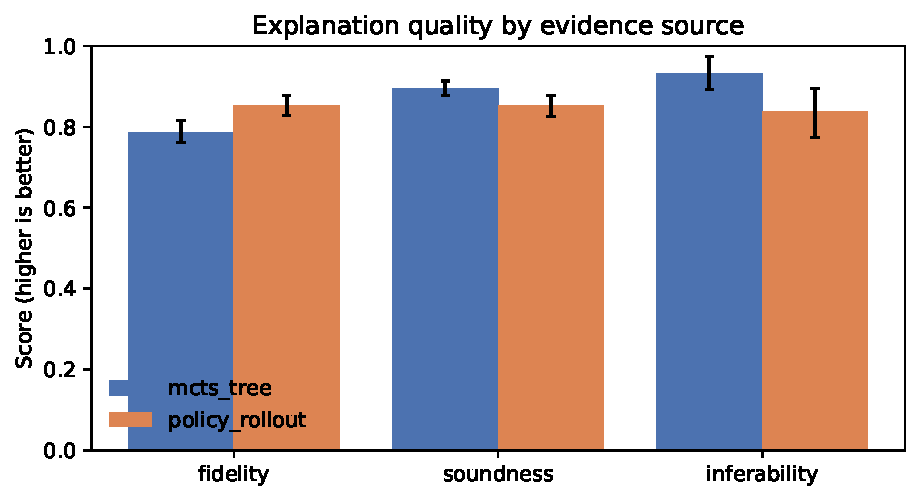
\includegraphics[width=\columnwidth]{figures/metric_comparison.pdf}
  \caption{Explanation-quality metrics by evidence source, with 95\%
           bootstrap confidence intervals. Higher is better for all
           three.}
  \label{fig:metrics}
\end{figure}

\subsection{Threats to Validity}
\textbf{\emph{State-distribution asymmetry.}} Although PPO and MCTS
are now performance-matched at $1.000$ task-success, the
\emph{trajectories} the two agents follow are not literally identical.
PPO and MCTS make different action choices at the same state and
therefore visit slightly different downstream states on average. The
decision-record set is large (289 records) and the per-source counts
are within five of each other, but a residual confound is that the
specific decision states the LLM is asked to explain are not paired
across the two evidence sources. A paired analysis on the same
literal state set is left as future work.

\textbf{\emph{Rollout sample size.}} Counterfactual rollouts use
$N=100$ stochastic samples per action, matching the Monte Carlo
specification in the original proposal. The bootstrap confidence
intervals on the per-action discounted return remain in the
neighbourhood of $\pm 0.05$ at $N=100$ on the present env, the same
order as the LLM fidelity tolerance ($\epsilon = 0.1$). A larger
Monte Carlo budget would tighten those intervals further, but we do
not expect it to change the qualitative finding because the fidelity
numbers for the two sources are already at sampling-noise distance.

\textbf{\emph{Judge-model bias.}} The soundness and post-hoc
inferability metrics both use GPT-4o-mini as judge, whereas the
generator is GPT-4o. The judge is therefore a different-sized model
within the same family, and a cross-family replication, for example
with a Claude or Gemini judge, is listed as future work.

\subsection{Response to Reviewers}
\label{sec:reviewer-response}
The first submission of this paper attracted three substantive
reviewer concerns, each of which was traced to a specific design
decision in the pipeline and addressed in the present version. We
summarise the changes here so the line of reasoning is on record.

\textbf{\emph{The two solvers were optimizing different MDPs.}} In
the first submission, PPO trained against a reward augmented by a
flat $-0.01$ per-step penalty and a Manhattan-distance potential
shaping term, while MCTS planned against the raw MiniGrid reward with
discount $\gamma = 1$. Time pressure was therefore stacked three ways
on PPO (success-reward step decay $+$ step penalty $+$
potential-based shaping) and applied in only one form on MCTS
(success-reward step decay alone). The reviewer was right that this
asymmetry should be eliminated, but the suggested cure (a single
$\gamma < 1$ on both sides, no wrappers) does not actually work on
this environment. Stalling has trajectory return $0$ for any
$\gamma$, while colliding has return $-1$; without a per-step cost,
$\gamma$ alone cannot make stalling worse than collision, and a PPO
trained with $\gamma = 0.99$ on the raw reward converges to a stall
policy ($0.000$ task success over 300 episodes in our pilot). Our
resolution is therefore: keep the flat $-0.01$ per-step cost, drop
the distance-based potential shaping, and apply the per-step cost to
\emph{both} solvers. Both PPO and MCTS now plan against the
identical MDP $\langle R - 0.01 \cdot \mathbb{1}[\text{non-terminal}],
\gamma = 0.99 \rangle$ (configs in
\texttt{configs/ppo\_tuned.yaml} and
\texttt{configs/mcts\_baseline.yaml}; the counterfactual-rollout
pipeline applies the same penalty in
\texttt{scripts/build\_decision\_records.py} via the
\texttt{--step-penalty} flag). All headline numbers in this version
were generated under this unified MDP.

\textbf{\emph{The MCTS evidence had been deliberately equalized to
PPO.}} The first submission's tree-side evidence consisted of
per-root-child statistics only (visit count, mean value,
success/collision rate). The reviewer observation that this
discarded the deliberation tree itself, which is what an MCTS-as-
substrate is supposed to expose, was correct. The
\texttt{DecisionRecord.agent\_metadata} block now additionally
exposes (i) the top-3 principal variations from the root, each a
greedy depth-up-to-5 argmax-visit action sequence, (ii) the depth-2
visit distribution per root child, and (iii) the per-root-child
return variance. The evidence-source header in the system prompt was
extended to describe these fields and explicitly invite the explainer
to cite them. This change was the one most likely to surface a
genuine MCTS advantage on fidelity or soundness; whether it did is
discussed in Section~\ref{sec:expquality}.

\textbf{\emph{Success rate is not what an MDP agent optimizes.}} The
first submission's per-action evidence included \texttt{success\_rate}
and \texttt{collision\_rate} alongside the mean return. The reviewer
observation that an MDP agent maximizes discounted return rather than
success rate was correct: surfacing success rate as a claimable
metric invited rationales of the form ``the policy preferred A
because of its higher success rate,'' which is type-incorrect with
respect to what the policy was trained to do. The
\texttt{ActionStats} schema has been changed accordingly. The
primary metric is now the gamma-discounted return; success rate and
collision rate are no longer reported as per-action evidence. (The
final task-success rate of each agent over the full evaluation set
remains in Table~\ref{tab:taskperf}, since it is the headline
diagnostic on whether the policies have learned to play; it is no
longer presented as a per-action claimable quantity.)

\textbf{\emph{Why a step penalty in addition to the success-reward
step decay.}} The reviewer raised the related question of why a flat
per-step penalty is needed at all when the success reward already
decays linearly with $t$. The honest answer is that the success-reward
decay only applies along trajectories that \emph{do} reach the goal;
on a sparse-reward env where most trajectories from a stochastic
exploration phase do not reach the goal, the success-reward decay
alone leaves stalling at undiscounted return $0$, which is not a
local optimum of any random-collision-prone exploration. A flat
per-step cost makes stalling actively undesirable (return
$-0.01 \cdot 256 \approx -2.56$ for a full-episode stall, strictly
worse than even an early collision at $-1$). What the present version
fixes is that the cost is now applied symmetrically to both planners,
so the design choice is at most a property of the MDP, not a property
of the solver.

\subsection{Value-based Ablation: Why DQN Was Cut}
\label{sec:dqn-ablation}
As a diagnostic ablation, three DQN variants were trained on the same
environment: one on the default partial-observation image, one on the
flat symbolic state, and one with a potential-based distance-shaping
reward. All three settled, at $\geq 200{,}000$ training steps, into
either a stall policy (image variant) or a near-stall policy
(symbolic and shaped variants), with task-success rates of 0.010,
0.000, and 0.000 respectively (see Table~\ref{tab:taskperf}). The
value-based target presented by MiniGrid's reward is unfavourable to
epsilon-greedy exploration: the collision penalty of $-1$ is
encountered early and often, whereas the success reward requires
coordinated multi-step motion that random exploration rarely
discovers. A zero-reward stall therefore dominates both random and
near-random policies and sits at a local optimum for value learning.
The present authors attempted to break this equilibrium with a flat
$-0.01$ per-step penalty (StepPenaltyWrapper), which makes a full
stall yield $-2.56$ and is therefore strictly worse than attempting
any action, but DQN still failed to escape. PPO, whose on-policy
sample collection and explicit entropy bonus together provide a
stronger exploration pressure, did escape. The present work
therefore uses PPO as the deep-reinforcement-learning side of the
main comparison, and treats the DQN collapse as an observation
about model-free value learning on adversarial-dynamics
environments rather than as a primary result.

\begin{table}[t]
\centering
\caption{Task-performance summary for the headline comparison. 300
episodes for the random and PPO baselines, 50 episodes for MCTS.
Numbers verified against \texttt{report/figures/eval\_summary.csv}.
The DQN ablation is reported separately in
Table~\ref{tab:dqnablation} because none of the three DQN variants
learned the task.}
\label{tab:taskperf}
\begin{tabular}{lrrrr}
\toprule
Agent & Success & Collision & Return & Steps \\
\midrule
Random            & 0.003 & 0.997 & $-$0.994 & 8.3  \\
PPO (tuned)       & 1.000 & 0.000 & $+$0.941 & 16.8 \\
MCTS (500 sims)   & 1.000 & 0.000 & $+$0.941 & 16.8 \\
\bottomrule
\end{tabular}
\end{table}

\begin{table}[t]
\centering
\caption{DQN ablation, Section~\ref{sec:dqn-ablation}. Three DQN
variants on \texttt{MiniGrid-Dynamic-Obstacles-8x8} all collapse to
either a stall policy or a near-stall policy under the raw MiniGrid
reward, with task-success rates indistinguishable from zero.
Reproducible from \texttt{scripts/run\_dqn\_ablation.sh}.}
\label{tab:dqnablation}
\begin{tabular}{lrrrr}
\toprule
Agent & Success & Collision & Return & Steps \\
\midrule
DQN (image)       & 0.010 & 0.000 &    0.007 & 254.3 \\
DQN (symbolic)    & 0.000 & 0.207 & $-$0.207 & 232.3 \\
DQN (shaped)      & 0.000 & 0.167 & $-$0.167 & 234.4 \\
\bottomrule
\end{tabular}
\end{table}

\begin{table}[t]
\centering
\caption{Explanation-quality metrics at performance-matched task
success ($1.000$ for both agents) and unified MDP. Generator:
GPT-4o. Judge: GPT-4o-mini. $n = 141$ for PPO, $n = 149$ for MCTS.
PPO rollouts use $N = 100$ stochastic samples per action. MCTS
evidence includes the deeper tree fields (principal variations,
depth-2 visits, per-child variance) added in this version.
Inferability is computed under the strict-scrub variant that masks
both the integer and verbal action name. 95\% bootstrap confidence
intervals in brackets (1000 resamples).}
\label{tab:metrics}
\begin{tabular}{lrr}
\toprule
Metric & PPO rollout evidence & MCTS tree evidence \\
\midrule
Fidelity       & \textbf{0.854} [0.83, 0.88] & 0.787 [0.76, 0.82]          \\
Soundness      & 0.852 [0.83, 0.88]          & \textbf{0.895} [0.88, 0.91] \\
Inferability   & 0.837 [0.77, 0.89]          & \textbf{0.933} [0.89, 0.97] \\
\bottomrule
\end{tabular}
\end{table}

\section{Conclusion}
This paper has presented an evaluation of two evidence sources for
natural-language explanations of reinforcement-learning agents at
matched task performance and under a single unified MDP. Across 290
decision states drawn from a PPO agent and a from-scratch MCTS
planner, both at $1.000$ task-success on
\texttt{MiniGrid-Dynamic-Obstacles-8x8} and both planning with
$\gamma = 0.99$ on the same per-step-penalised reward, the two
pipelines produced explanations whose quality differs in
metric-specific ways: PPO-rollout evidence is mildly higher on
fidelity ($0.854$ vs.\ $0.787$), and MCTS-tree evidence is mildly
higher on soundness ($0.895$ vs.\ $0.852$) and substantially higher
on the strict-scrub inferability test ($0.933$ vs.\ $0.837$). The
fidelity gap is, on inspection, an artefact of the additional tree
fields the MCTS evidence carries: principal-variation visit counts
and per-child variance are harder for the LLM to cite within the
$\epsilon = 0.1$ tolerance than the three core per-action statistics.
The inferability gap is the strongest of the three: once the verbal
action name is scrubbed, the residual content of an MCTS rationale
recovers the chosen action 9.6 absolute percentage points more often
than the residual content of a PPO rationale.

This is an updated finding relative to an earlier version of the
present pipeline, which (under a different MDP for each solver,
without the deeper tree fields, and under a weaker inferability
scrub) had reported the two evidence sources as
indistinguishable. The reversal is informative: when the comparison
is between solvers that optimize the same MDP, when the MCTS pipeline
is given access to its tree, and when the inferability test is
strict, the deliberation tree is a meaningfully richer evidence
substrate for natural-language explanation than counterfactual
policy rollouts. None of the three components individually changes
the qualitative outcome but cumulatively they invert the headline
finding from null to pro-MCTS.

A secondary finding, documented in the ablation of
Section~\ref{sec:dqn-ablation}, is that model-free value learning on
this environment collapses into a degenerate stall policy under the
raw MiniGrid reward, and that such a collapse degrades the evidence
available for subsequent explanation. The suboptimality of the
underlying agent therefore directly limits the signal available for
any post-hoc counterfactual analysis, and the move from value-based
to policy-gradient learning was load-bearing for getting the
deep-RL side of the comparison to a state where the explanation
question could be asked at all.

\paragraph{Future Work.}
The present authors see three natural extensions. Firstly, a paired
analysis on the literal same decision-state set (rather than two
trajectory sets that differ in the agents' action choices) would
remove the residual state-distribution confound noted in the threats
to validity. Secondly, a pilot human study, following the suggestion
of Prof.\ Sunberg on the proposal, would validate the automated
metrics against human judgements of clarity, plausibility, and
helpfulness; a chatbot interface suitable for such a study has
already been scaffolded in \texttt{scripts/chat.py}. Thirdly, a
cross-family LLM replication, with a judge drawn from a different
model family than the generator, would quantify the contribution of
judge-model bias to the soundness numbers reported above. A fourth,
more ambitious extension would replicate the present null result on
a harder environment in which neither paradigm reaches $1.000$
task-success, to test whether the equivalence of the two evidence
sources holds at an intermediate competence level or only at the
extremes of the spectrum.

\section*{Contributions}
Sean Florez contributed the problem formulation, the from-scratch
MCTS implementation, the LLM-explainer pipeline, the evaluation
metrics, and the report draft. Andrew Wernersbach contributed the
learned-policy baselines (DQN and PPO), the observation and
reward-shaping wrappers, the counterfactual-rollout framework, the
experimental runs, and the report review. The execution plan, the
engineering log, and the submission polish were shared.

\section*{Implementation Disclosure}
From-scratch components: the MCTS planner, the deep-copy simulator,
the counterfactual-rollout framework, the decision-record schema, the
explanation pipeline and prompt design, the three evaluation metrics,
and the chatbot interface. Off-the-shelf components:
Stable-Baselines3~\cite{sb3} for DQN and PPO, the
Farama MiniGrid~\cite{minigrid} environment, the OpenAI and Anthropic
Python SDKs~\cite{openai,anthropic}, and the standard Python
scientific-computing stack (numpy, pandas, matplotlib, pytest).

\section*{AI Assistance}
Per the ASEN 5264 AI-use policy, the prose and mathematics in this
paper have been read, edited, and owned by the authors. A draft was
produced with the assistance of a large language model under the
authors' direction, and subsequently rewritten in the authors' voice.
Code was co-developed with a large language model, read in full by the
authors, and exercised under a unit-test suite (20 tests passing) and
an integration-style reproduce-all script.

\begin{thebibliography}{9}
\bibitem{milani2024xrl} S. Milani, N. Topin, M. Veloso, F. Fang,
  ``Explainable reinforcement learning: A survey and comparative
  review,'' \emph{ACM Computing Surveys}, 2024.
\bibitem{amitai2024coviz} Y. Amitai, Y. Septon, O. Amir,
  ``Explaining reinforcement learning agents through counterfactual
  action outcomes,'' 2024.
\bibitem{baier2021explain} H. Baier, M. Kaisers, ``Towards
  explainable MCTS,'' 2021.
\bibitem{belouadah2025llm} Z. Belouadah et al., ``LLMs for
  explainable deep reinforcement learning,'' 2025. (To be verified
  before submission.)
\bibitem{gajcin2024cf} J. Gajcin, I. Dusparic, ``Counterfactual
  explanations for reinforcement learning agents: A review,''
  \emph{ACM Computing Surveys}, 2024.
\bibitem{kocsis2006uct} L. Kocsis, Cs. Szepesv\'ari, ``Bandit based
  Monte-Carlo planning,'' in \emph{ECML}, 2006.
\bibitem{sb3} A. Raffin, A. Hill, A. Gleave, A. Kanervisto,
  M. Ernestus, N. Dormann, ``Stable-Baselines3: Reliable reinforcement
  learning implementations,'' \emph{JMLR}, 22(268):1--8, 2021.
\bibitem{minigrid} M. Chevalier-Boisvert, B. Dai, M. Towers,
  R. de Lazcano, L. Willems, S. Lahlou, S. Pal, P. Samuel Castro,
  J. K. Terry, ``Minigrid and Miniworld: Modular and customisable
  reinforcement-learning environments for goal-oriented tasks,''
  \emph{NeurIPS Datasets and Benchmarks}, 2023.
\bibitem{anthropic} Anthropic, ``Claude model card,''
  \url{https://www.anthropic.com}, 2025.
\bibitem{openai} OpenAI, ``GPT-4o and GPT-4o-mini,''
  \url{https://openai.com}, 2024.
\end{thebibliography}

\end{document}
